% =============================================================================
%  Final report -- PostgreSQL optimisation project on the IMDb dataset.
%
%  Compile (from this directory):
%      xelatex -interaction=nonstopmode report.tex
%      xelatex -interaction=nonstopmode report.tex   (second pass: ToC/refs)
%
%  Requires: TeX Live / MiKTeX with xepersian, a Persian-capable system font.
%  B Nazanin itself is not installed on this machine (checked the Windows font
%  registry directly -- it is a commercial font not bundled with modern Windows
%  or TeX Live). Traditional Arabic is used instead: a classic Naskh-style
%  system font with a genuine bold weight, the closest available match to
%  B Nazanin's traditional look. If a real B Nazanin/Vazirmatn .ttf is ever
%  installed on the machine that compiles this, just change \settextfont below.
%  Arial is used for Latin text (plain, simple, no decorative serifs). The
%  Scale= factors below correct a real size mismatch: at the same nominal
%  point size, Traditional Arabic renders visibly smaller than most Latin
%  fonts, so Persian is scaled up and Latin scaled down to balance the two.
% =============================================================================
\documentclass[a4paper,12pt]{article}

% The bidi package (loaded by xepersian) requires several common packages --
% geometry, xcolor, array, longtable, listings, hyperref, among others -- to be
% loaded BEFORE it, or it raises a hard "Oops! you have loaded package X after
% bidi package" error. xepersian itself must therefore be the LAST \usepackage.
\usepackage{geometry}
\geometry{a4paper, margin=2.7cm}
\usepackage{xcolor}
\usepackage{graphicx}
\usepackage{booktabs}
\usepackage{longtable}
\usepackage{array}
\usepackage{listings}
\usepackage[xetex,unicode,colorlinks=true,linkcolor=blue!50!black,urlcolor=blue!50!black,citecolor=blue!50!black]{hyperref}

\usepackage{xepersian}
\settextfont[Scale=1.15]{Traditional Arabic}
\setlatintextfont[Scale=0.85]{Arial}
\setdigitfont[Scale=1.15]{Traditional Arabic}

% ---------------------------------------------------------------------------
%  Code listings: English source stays left-to-right even inside this
%  right-to-left document. Every \lstlisting below is wrapped in
%  \begin{latin}...\end{latin}, which is xepersian's own mechanism for
%  embedding Latin-script verbatim material (see xepersian.sty, \latin/\endlatin).
% ---------------------------------------------------------------------------
\lstdefinestyle{code}{
  basicstyle=\footnotesize\ttfamily,
  breaklines=true,
  breakatwhitespace=false,
  columns=fullflexible,
  keepspaces=true,
  frame=single,
  numbers=left,
  numberstyle=\tiny\color{gray},
  commentstyle=\color{gray}\itshape,
  keywordstyle=\color{blue!60!black}\bfseries,
  stringstyle=\color{orange!70!black},
  showstringspaces=false,
  tabsize=2,
  morekeywords={CREATE,INDEX,IF,NOT,EXISTS,ON,USING,GIN,WHERE,AND,SELECT,FROM,
    JOIN,LEFT,CROSS,LATERAL,GROUP,BY,ORDER,LIMIT,HAVING,WITH,PARTITION,OVER,
    RETURNS,LANGUAGE,plpgsql,AS,DECLARE,BEGIN,END,LOOP,FOR,UPDATE,SKIP,LOCKED,
    def,import,from,return,if,else,while,class,None,True,False},
}
\lstset{style=code}

% Long file/path references (e.g. scripts/compare_timings.py) need to stay
% left-to-right AND break gracefully at / and _ -- plain \lr{} has no break
% points and causes large overfull hboxes. \url (from the url package, loaded
% by hyperref) already breaks at exactly those characters, so \Rl reuses it.
\newcommand{\Rl}[1]{\url{#1}}

\author{}
\date{}

\begin{document}

% ---------------------------------------------------------------------------
%  Title page -- fill in the bracketed placeholders before submitting.
% ---------------------------------------------------------------------------
\begin{titlepage}
\centering
\vspace*{1.5cm}
{\Large دانشگاه صنعتی شریف}\\[2cm]

{\huge\bfseries بهینه‌سازی پایگاه‌داده \lr{PostgreSQL} برای مجموعه‌داده \lr{IMDb}}\\[0.5cm]
{\Large صف پیام، فشرده‌سازی \lr{TOAST} و ایندکس‌گذاری هدفمند}\\[2.5cm]

{\large درس: طراحی پایگاه داده -- نیم‌سال دوم سال تحصیلی 1404--1405}\\[0.3cm]
{\large استاد درس: دکتر رمضانی}\\[2cm]

{\large نگارش:}\\[0.4cm]
{\large سهیل سیاح ورگ -- \lr{402111237}}\\[0.2cm]
{\large امیرحسین موسوی فرد -- \lr{402111515}}\\[0.2cm]
{\large رضا اسلامی ابیانه -- \lr{402105619}}\\[1cm]

\vfill
\end{titlepage}

\section*{چکیده}

این گزارش درباره‌ی طراحی و بهینه‌سازی یک پایگاه‌داده \lr{PostgreSQL 16} برای مجموعه‌داده‌ی \lr{IMDb} است. این مجموعه‌داده خیلی بزرگ است -- حدود \lr{190} میلیون سطر در هفت جدول -- پس بارگذاری مستقیم آن هم کند است و هم فضای دیسک زیادی می‌گیرد. برای حل این مشکل، از یک \textbf{صف پیام} (\lr{message queue}) استفاده کردیم که با دستور \lr{SELECT ... FOR UPDATE SKIP LOCKED} کار می‌کند. این کار باعث می‌شود چند مصرف‌کننده هم‌زمان، بدون قفل‌شدن روی هم، داده را بنویسند. داده‌ها هم به‌صورت دسته‌ای (\lr{batch}) نوشته می‌شوند تا فشرده‌سازی \lr{TOAST} فعال شود و حجم روی دیسک کم شود.

بعد از بارگذاری، هشت کوئری تحلیلی که در سند پروژه خواسته شده بود را نوشتیم و اول بدون هیچ ایندکسی (خط پایه) با \lr{EXPLAIN (ANALYZE, BUFFERS)} بررسی کردیم. بعد شش ایندکس مناسب طراحی کردیم: چند \lr{B-Tree} جزئی برای فیلترهای بازه‌ای، و یک ایندکس \lr{GIN} ترکیبی (با کمک \lr{btree\_gin}) برای فیلتر روی \lr{title\_type}. طراحی ایندکس‌ها را با یک بازبینی خودکار چندعاملی بررسی کردیم و یک اسکریپت (\Rl{scripts/compare_timings.py}) هم نوشتیم که خودش جدول مقایسه‌ی «قبل/بعد» را از خروجی واقعی می‌سازد.

همه‌ی این پروژه -- بارگذاری، هشت سناریو، و ایندکس‌گذاری -- را واقعاً روی یک \lr{PostgreSQL 16} داخل \lr{Docker} اجرا کردیم. پس عددهای بخش \ref{sec:indexing} (زمان اجرا، تعداد بافر، نوع گره‌های پلن) واقعی‌اند، نه پیش‌بینی. فقط یک محدودیت وجود داشت: چون فضای دیسک سیستم اجرا کم بود، جدول \lr{title\_principals} فقط با \lr{8} میلیون از \lr{90} میلیون سطر واقعی‌اش بارگذاری شد (بخش \ref{sec:real-data-scale})؛ شش جدول دیگر کامل هستند. نتیجه هم یک‌دست نبود: شش سناریو سریع‌تر شدند، سناریوی \lr{3} تقریباً بدون تغییر ماند چون عمداً ایندکسی برایش نساختیم، و سناریوی \lr{1} با ایندکس \lr{GIN} حتی کندتر هم شد.


\tableofcontents
\newpage

\section{مقدمه}
\label{sec:intro}

\subsection{مسئله و انگیزه}

مجموعه‌داده‌ی \lr{IMDb} \cite{imdb, imdbdocs} یکی از بزرگ‌ترین مجموعه‌داده‌های رایگان در زمینه‌ی فیلم و سریال است. هفت جدول دارد که در مجموع نزدیک به \lr{190} میلیون سطر می‌شود (فقط جدول \lr{title\_principals} حدود \lr{90} میلیون سطر دارد). هدف این پروژه این است که یک پایگاه‌داده‌ی \lr{PostgreSQL 16} بسازیم که بتواند این حجم داده را هم از نظر فضای دیسک و هم از نظر سرعت کوئری، خوب مدیریت کند.

اگر بخواهیم فایل‌های \lr{TSV} فشرده را مستقیم و ساده بارگذاری کنیم (مثلاً با \lr{INSERT} تک‌تک یا حتی \lr{COPY} ساده)، دو مشکل پیش می‌آید:

\begin{enumerate}
\item \textbf{فضای دیسک.} اگر هر پیام فقط یک سطر باشد، اندازه‌ی آن از آستانه‌ی \lr{TOAST} (حدود \lr{2} کیلوبایت) رد نمی‌شود، یعنی ستون‌های \lr{JSONB} بدون فشرده‌سازی ذخیره می‌شوند. برای \lr{190} میلیون سطر، این چند ده گیگابایت فضای اضافه می‌شود که با محدودیت دیسک ما (حدود \lr{52} گیگابایت) جور در نمی‌آید.
\item \textbf{هم‌زمانی نوشتن.} می‌خواهیم چند پردازش هم‌زمان داده بنویسند تا سریع‌تر شود، اما اگر از قفل معمولی (\lr{FOR UPDATE} بدون \lr{SKIP LOCKED}) استفاده کنیم، همه پشت سر هم منتظر می‌مانند.
\end{enumerate}

راه‌حلی که انتخاب کردیم، گذاشتن یک صف پیام بین دانلود داده و درج نهایی است. یک تولیدکننده (\lr{producer}) فایل‌های فشرده را جریانی می‌خواند (بدون این‌که کامل روی دیسک استخراج شود)، سطرها را در دسته‌های \lr{1000}تایی بسته‌بندی و در صف می‌گذارد. یک یا چند مصرف‌کننده (\lr{consumer}) هم با \lr{SELECT ... FOR UPDATE SKIP LOCKED} \cite{pglocking} دسته‌ها را بدون رقابت با هم برمی‌دارند و با \lr{execute\_values} به‌صورت انبوه درج می‌کنند.

\subsection{اهداف گزارش}

این گزارش سه هدف دارد:

\begin{itemize}
\item توضیح کامل معماری پروژه: از تنظیمات \lr{PostgreSQL} و طراحی جدول‌ها تا صف پیام و خط لوله‌ی بارگذاری؛
\item نمایش و بررسی هشت سناریوی کوئری که سند پروژه خواسته، هم قبل از ایندکس‌گذاری و هم بعد از آن؛
\item پاسخ به سؤال‌های نظری پروژه درباره‌ی تنظیمات \lr{PostgreSQL}، انواع ایندکس، \lr{JSONB}/\lr{TOAST} و نظریه‌ی صف پیام.
\end{itemize}

\subsection{ساختار گزارش}

بخش \ref{sec:architecture} معماری اجرا و طراحی اسکیما را توضیح می‌دهد. بخش \ref{sec:queue} صف پیام و کد تولیدکننده/مصرف‌کننده را نشان می‌دهد. بخش \ref{sec:scenarios} هشت سناریوی کوئری را معرفی می‌کند. بخش \ref{sec:indexing} ایندکس‌ها و روش مقایسه‌ی عملکرد را توضیح می‌دهد. بخش \ref{sec:theory} به سؤال‌های نظری پاسخ می‌دهد و بخش \ref{sec:conclusion} جمع‌بندی است.

\section{معماری و محیط اجرا}
\label{sec:architecture}

\subsection{محیط اجرا: \lr{Docker Compose}}

پایگاه‌داده در یک کانتینر \lr{PostgreSQL 16} با \lr{docker-compose} اجرا می‌شود. جدول \ref{tab:pgconf} مهم‌ترین تنظیمات و دلیل هرکدام را نشان می‌دهد.

\begin{table}[h]
\centering
\caption{تنظیمات اصلی \lr{PostgreSQL} در \lr{docker-compose.yml}}
\label{tab:pgconf}
\begin{tabular}{@{}p{4.2cm}p{2.8cm}p{7cm}@{}}
\toprule
\textbf{پارامتر} & \textbf{مقدار} & \textbf{دلیل} \\
\midrule
\lr{shared\_buffers} & \lr{1536MB} & کش مشترک پایگاه‌داده؛ حدود یک‌چهارم تا یک‌سوم حافظه‌ی کل کانتینر (\lr{6GB}). \\
\lr{work\_mem} & \lr{32MB} (سراسری) & عمداً کم نگه داشته شده تا در خط پایه، ریزش (\lr{spill}) عملیات‌های \lr{Hash Join}/\lr{Sort} روی دیسک دیده شود؛ برای سناریوهای سنگین‌تر، اسکریپت اجرا این مقدار را فقط در سطح همان نشست بالا می‌برد. \\
\lr{effective\_cache\_size} & (متناسب با حافظه‌ی کل) & کمک می‌کند برنامه‌ریز کوئری تخمین بهتری از حافظه‌ی نهان سیستم‌عامل داشته باشد. \\
\lr{wal\_compression} & \lr{lz4} & رکوردهای \lr{WAL} را فشرده می‌کند تا حجم نوشتار دیسک کمتر شود. \\
\Rl{default_toast_compression} & \lr{lz4} & فشرده‌سازی پیش‌فرض \lr{TOAST} برای ستون‌های متغیرطول. \\
\lr{jit} & \lr{off} & چون کوئری‌های این پروژه تحلیلی و کوتاه‌مدت‌اند، خاموش‌کردن \lr{JIT} برنامه‌ریزی را پیش‌بینی‌پذیرتر می‌کند. \\
\lr{track\_io\_timing} & \lr{on} & تا \lr{EXPLAIN (BUFFERS)} بتواند زمان واقعی \lr{I/O} را هم نشان دهد. \\
\Rl{shared_preload_libraries} & \Rl{pg_stat_statements} & برای جمع‌آوری آمار هر کوئری. \\
\bottomrule
\end{tabular}
\end{table}

کانتینر با محدودیت حافظه‌ی \lr{6GB} و \lr{shm\_size} برابر \lr{1GB} اجرا می‌شود. داده هم روی یک والیوم نام‌گذاری‌شده (\lr{pgdata}) ذخیره می‌شود تا با ری‌استارت کانتینر از بین نرود.

\subsection{طراحی اسکیما}

هفت جدول اصلی \lr{IMDb} در اسکیمای \lr{imdb} تعریف شده‌اند: \lr{title\_basics}، \lr{title\_ratings}، \lr{title\_crew}، \lr{title\_episode}، \lr{name\_basics}، \lr{title\_principals} و \lr{title\_akas}. اسم ستون‌ها هم \lr{snake\_case} شده‌ی همان اسم‌های \lr{camelCase} فایل‌های اصلی \lr{TSV} است.

سه نکته‌ی طراحی مهم:

\begin{enumerate}
\item \textbf{ستون \lr{metadata JSONB} روی هر جدول.} هر جدول یک ستون \lr{JSONB} قابل‌تهی دارد که هم برای نگه‌داشتن داده‌ی مشتق‌شده (مثلاً دسته‌بندی امتیاز در \lr{title\_ratings}) و هم برای نشان‌دادن عملیِ مکانیزم \lr{TOAST} استفاده می‌شود. روی دو جدول بزرگ (\lr{title\_principals} و \lr{title\_akas}) این ستون همیشه \lr{NULL} می‌ماند.

\item \textbf{بدون کلید خارجی در ابتدا.} چون پیام‌ها ممکن است خارج از ترتیب از صف بیرون بیایند (مثلاً یک سطر \lr{title\_ratings} قبل از سطر والدش در \lr{title\_basics} برسد)، اگر از اول کلید خارجی بگذاریم، درج‌های درست هم شکست می‌خورند؛ ضمن این‌که یک بررسی ایندکسی اضافه به ازای هر سطر، روی یک بارگذاری \lr{190} میلیون سطری هزینه‌ی زیادی دارد. به همین دلیل کلید خارجی را بعد از تمام‌شدن بارگذاری، به‌صورت \lr{NOT VALID} و بعد \lr{VALIDATE CONSTRAINT}، اضافه می‌کنیم.

\item \textbf{ترتیب فیلدها در \lr{title\_principals}.} ستون عددی \lr{ordering} قبل از ستون‌های متنی نوشته شده. چون ترتیب فیلدها در \lr{PostgreSQL} دقیقاً همان ترتیب اعلامشان است، اگر یک عدد \lr{4}بایتی بعد از یک رشته‌ی کوتاه بیاید، باز هم باید هم‌ترازیِ \lr{4}بایتی رعایت شود و تا \lr{3} بایت در هر سطر هدر می‌رود. روی \lr{90} میلیون سطر، این یعنی حدود \lr{150} مگابایت فضای اضافه که با تغییر ترتیب حذف می‌شود.
\end{enumerate}

سه افزونه هم در راه‌اندازی اولیه فعال می‌شوند: \lr{pg\_stat\_statements} (آمار هر کوئری)، \lr{btree\_gin} (که در بخش \ref{sec:indexing} برای ساخت یک ایندکس \lr{GIN} ترکیبی استفاده می‌شود)، و \lr{pgstattuple} (برای اندازه‌گیری واقعی نسبت فشرده‌سازی \lr{TOAST}).

\section{صف پیام و بارگذاری جریانی}
\label{sec:queue}

\subsection{جدول صف پیام}

هسته‌ی خط لوله‌ی بارگذاری، جدولی به اسم \lr{message\_queue} است که مثل یک صف کار عمل می‌کند:

\begin{latin}
\begin{lstlisting}[language=SQL, caption={message\_queue table structure}]
CREATE TABLE imdb.message_queue (
    id           BIGINT      GENERATED ALWAYS AS IDENTITY,
    attempts     INTEGER     NOT NULL DEFAULT 0,
    queue_name   TEXT        NOT NULL,
    status       TEXT        NOT NULL DEFAULT 'pending',
    payload      JSONB       NOT NULL,
    last_error   TEXT,
    locked_until TIMESTAMPTZ,
    created_at   TIMESTAMPTZ NOT NULL DEFAULT now(),
    updated_at   TIMESTAMPTZ NOT NULL DEFAULT now(),
    CONSTRAINT message_queue_pkey PRIMARY KEY (id),
    CONSTRAINT message_queue_status_chk
        CHECK (status IN ('pending', 'processing', 'done', 'failed'))
);

-- Only claimable rows need to be found fast; 'done' rows drop out entirely.
CREATE INDEX message_queue_ready_idx
    ON imdb.message_queue (queue_name, id) WHERE status = 'pending';

-- Used by the reaper that returns expired leases to 'pending'.
CREATE INDEX message_queue_stuck_idx
    ON imdb.message_queue (locked_until) WHERE status = 'processing';
\end{lstlisting}
\end{latin}

هر پیام یکی از چهار وضعیت را دارد: \lr{pending}، \lr{processing}، \lr{done} یا \lr{failed}. دو ایندکس جزئی روی این جدول گذاشته‌ایم: \lr{message\_queue\_ready\_idx} فقط سطرهای \lr{pending} را در بر می‌گیرد (پس اندازه‌اش با تعداد کارهای باقی‌مانده رشد می‌کند، نه با کل تاریخچه‌ی صف)، و \lr{message\_queue\_stuck\_idx} برای پیدا کردن پیام‌هایی که مهلتشان تمام شده استفاده می‌شود. جدول با \lr{fillfactor = 80} ساخته شده چون هر پیام حداقل دو بار آپدیت می‌شود (یک‌بار وقتی برداشته می‌شود، یک‌بار وقتی تأیید می‌شود). \lr{autovacuum} هم روی این جدول با آستانه‌ی مطلق تنظیم شده، چون یک صف خیلی سریع‌تر از آستانه‌ی پیش‌فرض \lr{20\%} سطر مرده تولید می‌کند.

\subsection{توابع \lr{PL/pgSQL} صف}

پنج تابع اصلی روی این جدول نوشته‌ایم:

\begin{itemize}
\item \lr{enqueue} و \lr{enqueue\_many}: اضافه‌کردن یک یا چند پیام؛
\item \lr{dequeue}: برداشتن یک دسته از پیام‌های \lr{pending} با \lr{SELECT ... FOR UPDATE SKIP LOCKED} \cite{pglocking} و علامت‌زدن آن‌ها به \lr{processing} با یک مهلت؛
\item \lr{ack}: علامت‌زدن یک پیام به \lr{done} بعد از پردازش موفق؛
\item \lr{nack}: زیاد کردن شمارنده‌ی تلاش؛ اگر هنوز به سقف نرسیده، پیام دوباره \lr{pending} می‌شود، وگرنه \lr{failed} می‌شود؛
\item \lr{reap\_expired}: پیام‌هایی که در \lr{processing} گیر کرده‌اند (یعنی مصرف‌کننده‌شان قبل از تأیید یا رد کردن از کار افتاده) را دوباره \lr{pending} می‌کند.
\end{itemize}

\begin{latin}
\begin{lstlisting}[language=SQL, caption={Core of dequeue(): lock-free batch claim}]
WITH claimed AS (
    SELECT id
    FROM   imdb.message_queue
    WHERE  queue_name = p_queue_name AND status = 'pending'
    ORDER  BY id
    FOR UPDATE SKIP LOCKED
    LIMIT  p_batch_size
)
UPDATE imdb.message_queue mq
SET    status = 'processing',
       locked_until = now() + p_visibility_timeout,
       attempts = attempts + 1,
       updated_at = now()
FROM   claimed
WHERE  mq.id = claimed.id
RETURNING mq.id, mq.payload;
\end{lstlisting}
\end{latin}

نکته‌ی مهم \lr{SKIP LOCKED} این است: اگر چند مصرف‌کننده هم‌زمان این کوئری را اجرا کنند، هرکدام سطرهایی که مصرف‌کننده‌ی دیگر قبلاً قفل کرده را رد می‌کند و می‌رود سراغ سطر بعدی که آزاد است. یعنی به‌جای این‌که منتظر بمانند، هرکدام یک دسته‌ی جدا از صف برمی‌دارند -- دقیقاً همان چیزی که الگوی \lr{Competing Consumers} لازم دارد (توضیح کامل‌تر در بخش \ref{sec:theory}).

سه تابع باقی‌مانده -- \lr{enqueue}، \lr{ack} و \lr{nack} -- ساده‌ترند: هرکدام یک \lr{INSERT}/\lr{UPDATE} تک‌سطری روی \lr{message\_queue} هستند. هسته‌ی هرکدام (بدون بخش‌های اعتبارسنجی ورودی) این‌طور است:

\begin{latin}
\begin{lstlisting}[language=SQL, caption={Core of enqueue(), ack() and nack()}]
-- enqueue(): append one message
INSERT INTO imdb.message_queue (queue_name, payload)
VALUES (p_queue_name, p_payload)
RETURNING id INTO v_id;

-- ack(): processing -> done, only if this worker's lease is still valid
UPDATE imdb.message_queue mq
SET    status = 'done', locked_until = NULL, updated_at = now()
WHERE  mq.id = p_message_id AND mq.status = 'processing';
GET DIAGNOSTICS v_rows = ROW_COUNT;
RETURN v_rows = 1;   -- FALSE means the lease had already expired

-- nack(): count the failure; retry while under the cap, else park as 'failed'
UPDATE imdb.message_queue mq
SET    attempts     = mq.attempts + 1,
       last_error   = left(coalesce(p_error_message, ''), 2000),
       status       = CASE WHEN mq.attempts + 1 >= p_max_attempts
                           THEN 'failed' ELSE 'pending' END,
       locked_until = NULL, updated_at = now()
WHERE  mq.id = p_message_id AND mq.status = 'processing'
RETURNING mq.status INTO v_status;
\end{lstlisting}
\end{latin}

\lr{ack} مقدار \lr{BOOLEAN} برمی‌گرداند (نه \lr{VOID} مثل اسکلت اولیه‌ی سند پروژه): \lr{FALSE} یعنی مهلت پیام قبل از تأیید تمام شده و احتمالاً یک مصرف‌کننده‌ی دیگر همان پیام را دوباره پردازش کرده -- بی‌ضرر است چون درج‌ها \lr{ON CONFLICT DO NOTHING} دارند. کد کامل و تست‌شده‌ی هر پنج تابع (به‌همراه \lr{reap\_expired}، \lr{queue\_stats} و \lr{purge\_done}) در \Rl{sql/01_queue_functions.sql} است.

\subsection{بسته‌بندی دسته‌ای و آستانه‌ی \lr{TOAST}}

فشرده‌سازی \lr{TOAST} در \lr{PostgreSQL} \cite{pgtoast} بر اساس هر سطر (تاپل) فعال می‌شود، نه هر ستون. یعنی فقط وقتی کل اندازه‌ی یک سطر از آستانه‌ی \lr{TOAST\_TUPLE\_THRESHOLD} (حدود \lr{2} کیلوبایت) بیشتر شود، \lr{PostgreSQL} شروع به فشرده‌کردن و بیرون‌بردن ستون‌های بزرگ می‌کند. اگر هر پیام فقط یک سطر باشد (حدود \lr{200} بایت)، این آستانه هیچ‌وقت رد نمی‌شود و \lr{JSONB} بدون فشرده‌سازی ذخیره می‌شود -- برای \lr{190} میلیون پیام، این یعنی چند ده گیگابایت فضای اضافه.

راه‌حل این است که \lr{1000} سطر را در یک پیام بسته‌بندی کنیم:

\begin{latin}
\begin{lstlisting}[language=Python, caption={Two message payload shapes}]
# single : {"table": "title_basics", "data": {...}}          <- one row
# batch  : {"table": "title_basics", "rows": [{...}, ...]}   <- 1000 rows
\end{lstlisting}
\end{latin}

بار یک دسته‌ی \lr{1000}تایی چند صد کیلوبایت است، یعنی از آستانه رد می‌شود، پس با \lr{lz4} فشرده و به \lr{TOAST} منتقل می‌شود. چون کلیدهای \lr{JSON} در همه‌ی سطرها تکرار می‌شوند، فشرده‌سازی خیلی خوب کار می‌کند. سربار هدر هر سطر (\lr{24} بایت) هم به همین نسبت \lr{1000} برابر کم می‌شود. این ادعا را روی داده‌ی واقعی این پروژه هم اندازه‌گیری کردیم. با \lr{pg\_column\_size} (اندازه‌ی واقعی روی دیسک) در برابر طول متن خام \lr{JSON} هر پیام، روی \lr{1{,}079} پیام باقی‌مانده در \lr{message\_queue} حساب کردیم: \lr{113} مگابایت خام به فقط \lr{20} مگابایت رسید. یعنی نسبت فشرده‌سازی واقعی \lr{5.72} برابر. خود جدول \lr{message\_queue} هم همین را نشان می‌دهد: بخش اصلی سطر (\lr{heap}) فقط \lr{424} کیلوبایت است، ولی بخش \lr{TOAST} آن \lr{48} مگابایت -- دقیقاً همان چیزی که از طراحی بسته‌بندی دسته‌ای انتظار داشتیم.

\subsection{تولیدکننده (\lr{Producer})}

تولیدکننده (\Rl{scripts/producer.py}) فایل‌های فشرده‌ی \lr{.tsv.gz} را جریانی می‌خواند، یعنی هیچ‌وقت نسخه‌ی استخراج‌شده‌ی کامل را روی دیسک نمی‌نویسد. سطرها را با تابع مناسب هر ستون تبدیل می‌کند (عدد کوچک، بولی، آرایه، \lr{JSON})، در دسته‌های \lr{1000}تایی بسته‌بندی و با \Rl{enqueue_many} در صف می‌گذارد. یک مکانیزم فشار-پس (\lr{backpressure}) هم با پرس‌وجوی دوره‌ای \Rl{queue_stats} جلوی رشد زیاد صف را می‌گیرد: اگر تعداد پیام‌های \lr{pending} از یک حد بیشتر شود، تولیدکننده کمی کندتر می‌شود.

بخش اصلی کد -- ساخت بار پیام و ارسال آن به تابع صف -- این‌طور است:

\begin{latin}
\begin{lstlisting}[language=Python, caption={scripts/producer.py -- payload shaping and enqueue call}]
def make_payloads(table, rows, shape):
    dumps = lambda o: json.dumps(o, separators=(",", ":"), ensure_ascii=False)
    if shape == "single":
        return [dumps({"table": table, "data": r}) for r in rows]
    return [dumps({"table": table, "rows": rows})]     # 1000-row batch shape

def emit(self, payloads):
    with self.data.cursor() as cur:
        if self.args.enqueue_mode == "single" or len(payloads) == 1:
            for p in payloads:
                cur.execute("SELECT imdb.enqueue(%s, %s::jsonb)", (self.queue, p))
        else:
            cur.execute(
                "SELECT count(*) FROM imdb.enqueue_many"
                "(%s, ARRAY(SELECT jsonb_array_elements(%s::jsonb)))",
                (self.queue, "[" + ",".join(payloads) + "]"))
    self.messages_since_commit += len(payloads)
\end{lstlisting}
\end{latin}

\subsection{مصرف‌کننده (\lr{Consumer})}

مصرف‌کننده (\Rl{scripts/consumer.py}) با \lr{dequeue} دسته‌ها را برمی‌دارد، هر دو شکل بار پیام را می‌فهمد، و با \lr{execute\_values} درج انبوه می‌کند. اگر یک سطر خراب درون یک دسته باشد، برای این‌که کل دسته خراب نشود، هر دسته درون یک \lr{SAVEPOINT} اجرا می‌شود. اگر درج انبوه شکست بخورد، مصرف‌کننده به یک مسیر سطر-به-سطر برمی‌گردد تا فقط همان سطر خراب را در جدول \lr{dead\_letter} بگذارد و بقیه‌ی دسته درست درج شود. یک نخ جدا هم به‌طور دوره‌ای \lr{reap\_expired} را صدا می‌زند تا پیام‌هایی که مصرف‌کننده‌شان از کار افتاده، دوباره به صف برگردند -- این همان چیزی است که تضمین \textbf{حداقل یک‌بار تحویل} را می‌سازد (توضیح کامل در بخش \ref{sec:theory}).

حلقه‌ی اصلی هر کارگر (ساده‌شده؛ منطق اتصال‌مجدد و خاموش‌شدن امن حذف شده) این‌طور است:

\begin{latin}
\begin{lstlisting}[language=Python, caption={scripts/consumer.py -- main worker loop (simplified)}]
while not SHUTDOWN.is_set():
    messages = dequeue(lease, args.queue, args.batch, args.visibility)
    if not messages:
        wait_shutdown(args.poll)
        continue

    for msg_id, payload in messages:
        table, rows = split_payload(payload)
        res = ingest_message(work, table, rows)   # execute_values inside a SAVEPOINT
        if res["action"] == "ack":
            ack(lease, msg_id)
        else:
            nack(lease, msg_id, res["error"] or "", args.max_attempts)
\end{lstlisting}
\end{latin}

اگر \lr{execute\_values} روی کل دسته خطا بدهد (نه یک خطای موقتی مثل \lr{deadlock})، \lr{ingest\_message} به همان دسته با \lr{SAVEPOINT} جدا برای هر سطر برمی‌گردد؛ فقط سطرهای واقعاً خراب به \lr{dead\_letter} می‌روند و بقیه با موفقیت درج می‌شوند.

\section{سناریوهای کوئری و خط پایه}
\label{sec:scenarios}

\subsection{هشت سناریوی گزارش}

طبق سند پروژه، هشت کوئری تحلیلی روی داده تعریف و در فایل \Rl{sql/04_scenarios.sql} نوشته شده‌اند. جدول \ref{tab:scenarios} خلاصه‌ی آن‌هاست؛ همه از \lr{CROSS JOIN LATERAL unnest(...)} برای باز کردن ستون‌های آرایه‌ای (\lr{genres}، \lr{directors}) استفاده می‌کنند.

\begin{table}[h]
\centering
\caption{هشت سناریوی کوئری گزارش}
\label{tab:scenarios}
\begin{tabular}{@{}p{0.7cm}p{6cm}p{7.3cm}@{}}
\toprule
\textbf{\#} & \textbf{عنوان} & \textbf{ویژگی اصلی} \\
\midrule
\lr{1} & میانگین امتیاز فیلم به تفکیک ژانر & \lr{unnest(genres)}، پیوند با \lr{title\_ratings} \\
\lr{2} & \lr{10} فیلم برتر بر اساس تعداد رأی (حداقل \lr{1000} رأی) & \lr{ORDER BY num\_votes DESC LIMIT 10} \\
\lr{3} & \lr{20} کارگردان برتر بر اساس تعداد فیلم و میانگین امتیاز & \lr{unnest(directors)}، \lr{LEFT JOIN} به امتیازها \\
\lr{4} & میانگین امتیاز سالانه از سال \lr{2000} به بعد & فیلتر بازه‌ای روی \lr{start\_year} \\
\lr{5} & بازیگرانی با بیش از \lr{5} ژانر متفاوت & سنگین‌ترین کوئری؛ از \lr{title\_principals} (\lr{~90M} سطر) شروع می‌شود \\
\lr{6} & سریال‌هایی با بیشترین تعداد فصل & پیوند \lr{title\_episode} به والد از طریق \lr{parent\_tconst} \\
\lr{7} & پرتکرارترین جفت ژانر هم‌زمان & خودپیوندِ دو \lr{unnest} با \lr{g1.genre < g2.genre} \\
\lr{8} & \lr{5} فیلم بلندتر در هر ژانر & تابع پنجره‌ای \lr{ROW\_NUMBER() OVER (PARTITION BY genre ...)} \\
\bottomrule
\end{tabular}
\end{table}

برای نمونه، سناریوی \lr{1} (که خود سند پروژه هم آن را مثال زده) این‌طور است:

\begin{latin}
\begin{lstlisting}[language=SQL, caption={Scenario 1: average rating by genre}]
SELECT g.genre,
       ROUND(AVG(tr.average_rating), 2) AS avg_rating,
       COUNT(*)                         AS rated_titles
FROM   imdb.title_basics tb
CROSS  JOIN LATERAL unnest(tb.genres) AS g(genre)
JOIN   imdb.title_ratings tr ON tr.tconst = tb.tconst
WHERE  tb.title_type = 'movie'
GROUP  BY g.genre
ORDER  BY AVG(tr.average_rating) DESC;
\end{lstlisting}
\end{latin}

\subsection{رفتار مورد انتظار در خط پایه}

قبل از هر ایندکس‌گذاری (بخش \ref{sec:indexing})، فقط کلیدهای اصلی ایندکس دارند. این یعنی:

\begin{itemize}
\item \textbf{اسکن ترتیبی همه‌جا.} چون شرط‌هایی مثل \lr{title\_type = 'movie'} یا \lr{num\_votes >= 1000} هیچ ایندکسی ندارند، برنامه‌ریز مجبور است کل جدول را بخواند و سطر به سطر فیلتر کند. روی جدول‌های بزرگ (\lr{title\_basics} حدود \lr{12} میلیون سطر، \lr{title\_principals} حدود \lr{90} میلیون سطر)، این به‌صورت \lr{Parallel Seq Scan} دیده می‌شود.
\item \textbf{پیوند درهم (\lr{Hash Join}) با ریزش روی دیسک.} چون \lr{work\_mem} سراسری روی \lr{32MB} نگه داشته شده، اگر جدول هش یک پیوند از این مقدار بزرگ‌تر شود، به چند \lr{batch} روی دیسک می‌شکند.
\item \textbf{تجمیع و مرتب‌سازی ریزشی.} \lr{HashAggregate} و \lr{Sort} هم وقتی از \lr{work\_mem} بزرگ‌تر شوند، روی دیسک ریزش می‌کنند.
\item \textbf{از نظر طراحی، سناریوی \lr{5} باید سنگین‌ترین باشد.} این سناریو از \lr{title\_principals} شروع می‌شود که به‌طور طبیعی بزرگ‌ترین جدول این پروژه است (نزدیک \lr{90} میلیون سطر). بعد به \lr{title\_basics} و \lr{name\_basics} پیوند می‌خورد، ژانرها باز می‌شوند، و در آخر \lr{COUNT(DISTINCT genre)} گرفته می‌شود. پس انتظار داریم این کوئری بیشترین فایل موقت و بیشترین زمان را در خط پایه داشته باشد. اما در اجرای واقعی این پروژه، \lr{title\_principals} به‌خاطر محدودیت فضای دیسک فقط با \lr{8} میلیون سطر (حدود \lr{9\%} حجم واقعی) بارگذاری شد (جزئیات در بخش \ref{sec:real-data-scale})؛ درعوض \lr{title\_crew} و \lr{name\_basics} کامل ماندند. به همین دلیل سناریوی \lr{3} -- که از این دو جدول کامل می‌خواند -- در عمل سنگین‌تر از سناریوی \lr{5} از آب درآمد. این خودش یک نمونه‌ی خوب است: همیشه باید با عدد واقعی سنجید، نه فقط با اندازه‌ی نظری جدول.
\end{itemize}

قبل از اندازه‌گیری خط پایه، دستور \lr{ANALYZE} روی هر هفت جدول اجرا می‌شود. بلافاصله بعد از یک بارگذاری انبوه، آمار برنامه‌ریز خالی است (\lr{reltuples = -1})؛ بدون این آمار، برنامه‌ریز اندازه‌ی پیوندها را الکی حدس می‌زند و پلن‌های خیلی بد و غیرقابل‌تکرار انتخاب می‌کند. اجرای \lr{ANALYZE} این آمار را تازه می‌کند تا عدد «قبل از بهینه‌سازی» معنا داشته باشد.

اجرای این اندازه‌گیری‌ها با \Rl{scripts/run_scenarios.py} خودکار شده است: این اسکریپت \lr{ANALYZE} را اجرا می‌کند، برای هر سناریو خروجی \lr{EXPLAIN (ANALYZE, BUFFERS, SETTINGS)} را در \Rl{results/explain/} می‌نویسد، و زمان اجرا را در \Rl{results/timings/scenario_timings.csv} ثبت می‌کند.

شکل \ref{fig:success} یک اجرای واقعی و موفق را نشان می‌دهد: هر دو کانتینر \lr{Docker} در حال اجرا هستند، و سناریوی \lr{2} با ایندکس واقعی \lr{idx\_title\_ratings\_votes\_desc} به‌جای \lr{Seq Scan} از \lr{Index Scan} استفاده می‌کند.

\begin{figure}[h]
\centering
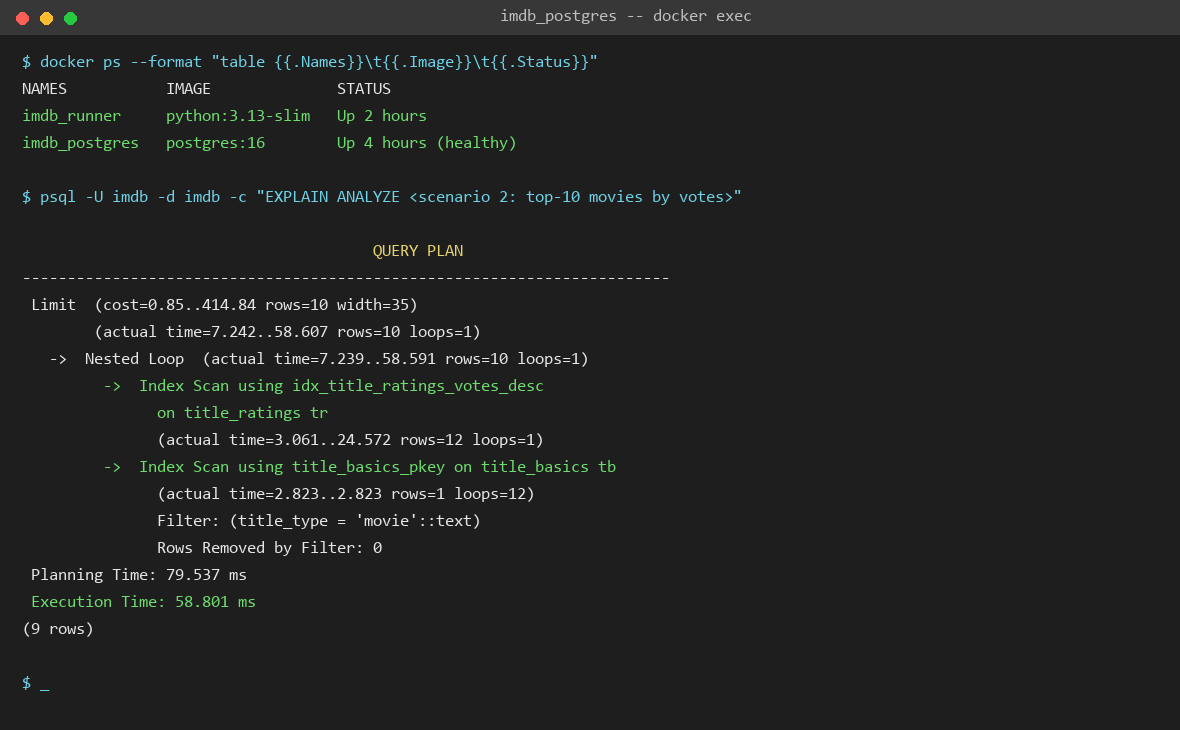
\includegraphics[width=0.85\linewidth]{figures/successful_execution.png}
\caption{اجرای موفق: کانتینرهای \lr{Docker} در حال کار، و \lr{EXPLAIN ANALYZE} واقعی سناریوی \lr{2} بعد از ایندکس‌گذاری}
\label{fig:success}
\end{figure}

\section{استراتژی ایندکس‌گذاری و تحلیل عملکرد}
\label{sec:indexing}

\subsection{اصل طراحی}

هر ایندکس در \Rl{sql/03_indexes.sql} به یک شرط \lr{WHERE}/\lr{ORDER BY}/\lr{JOIN} مشخص در یکی از هشت سناریوی بخش \ref{sec:scenarios} وصل است. هیچ ایندکسی «برای احتیاط» اضافه نشده، چون هر ایندکس هزینه‌ی نوشتاری (رکورد \lr{WAL}، شکافتن صفحه، کار \lr{autovacuum}) به هر \lr{INSERT}/\lr{UPDATE} بعدی آن جدول اضافه می‌کند. همه‌ی شش ایندکس زیر بعد از بارگذاری انبوه (بخش‌های قبلی) ساخته می‌شوند -- همان ترتیب معمول «اول بارگذاری، بعد ایندکس».

\subsection{شش ایندکس هدفمند}

\begin{latin}
\begin{lstlisting}[language=SQL, caption={sql/03\_indexes.sql -- summary}]
-- 1. Composite GIN: title_type (scalar, via btree_gin) + genres (array).
CREATE INDEX idx_title_basics_type_genres_gin
    ON imdb.title_basics USING GIN (title_type, genres);

-- 2. Partial B-tree, scoped to movies -- serves scenario 4.
CREATE INDEX idx_title_basics_movie_year
    ON imdb.title_basics (start_year) WHERE title_type = 'movie';

-- 3. Partial B-tree, scoped to movies with a known runtime -- scenario 8.
CREATE INDEX idx_title_basics_movie_runtime
    ON imdb.title_basics (runtime_minutes)
    WHERE title_type = 'movie' AND runtime_minutes IS NOT NULL;

-- 4. Partial B-tree for Top-N by votes -- scenario 2.
CREATE INDEX idx_title_ratings_votes_desc
    ON imdb.title_ratings (num_votes DESC) WHERE num_votes >= 1000;

-- 5. Partial composite B-tree, scoped to acting credits -- scenario 5.
CREATE INDEX idx_title_principals_cast
    ON imdb.title_principals (nconst, tconst)
    WHERE category IN ('actor', 'actress');

-- 6. Partial composite B-tree, scoped to numbered episodes -- scenario 6.
CREATE INDEX idx_title_episode_parent
    ON imdb.title_episode (parent_tconst, season_number)
    WHERE season_number IS NOT NULL;
\end{lstlisting}
\end{latin}

\paragraph{ایندکس \lr{1} (\lr{GIN} ترکیبی).} سناریوهای \lr{1}، \lr{3}، \lr{5} و \lr{7} همگی روی \lr{title\_type = 'movie'} فیلتر می‌کنند، اما هیچ‌کدام ژانرها را با مقدار خاصی فیلتر نمی‌کنند -- همه‌ی ژانرهای هر سطر را با \lr{unnest()} باز و بعد گروه‌بندی می‌کنند. یک ایندکس \lr{GIN} فقط برای سؤال «آیا این آرایه شامل مقدار \lr{X} است؟» سریع است، نه برای «همه‌ی مقادیر این آرایه را بده» -- پس یک \lr{GIN} تنها روی \lr{genres} هیچ سودی برای این هشت کوئری ندارد. راه‌حلی که انتخاب کردیم از یک ویژگی مستند \lr{GIN} \cite{pggin} استفاده می‌کند: برخلاف \lr{B-Tree} که فقط ستون اول قابل‌استفاده است، یک ایندکس \lr{GIN} چندستونی را می‌شود با فیلتر روی هرکدام از ستون‌هایش هم استفاده کرد. با ترکیب \lr{title\_type} (با کمک \lr{btree\_gin}) و \lr{genres} در یک ایندکس، همین یک ایندکس هم فیلتر \lr{title\_type = 'movie'} را جواب می‌دهد و هم برای سؤال‌های آینده مثل «همه‌ی فیلم‌های کمدی» رایگان کار می‌کند.

\paragraph{ایندکس‌های \lr{2} و \lr{3} (بازه‌ای، جزئی).} \lr{GIN} مفهوم ترتیب ندارد، پس نمی‌تواند شرط بازه‌ای مثل \lr{>= 2000} را جواب دهد -- \lr{B-Tree} ساختار درست برای این حالت است. شرط \lr{WHERE} جزئی هم دقیقاً همان شرط \lr{title\_type = 'movie'} سناریوهای \lr{4} و \lr{8} را تکرار می‌کند تا برنامه‌ریز مجبور نباشد آن را برای هر سطر دوباره چک کند.

\paragraph{ایندکس \lr{4} (\lr{Top-N}).} این یک مثال کلاسیک «ایندکس برای \lr{Top-N}» است: با این ایندکس، پلن به یک اسکن ایندکسی از بالاترین \lr{num\_votes} به پایین تبدیل می‌شود که هر سطر را برای \lr{title\_type = 'movie'} چک می‌کند و به‌محض رسیدن به \lr{LIMIT 10} متوقف می‌شود -- به‌جای این‌که همه‌ی عنوان‌های امتیازدهی‌شده را مرتب کند.

\paragraph{ایندکس \lr{5} (سنگین‌ترین سناریو).} \lr{category} حدود ده مقدار متفاوت دارد (\lr{actor}، \lr{actress}، \lr{director}، ...)؛ محدودکردن ایندکس به \lr{actor}/\lr{actress} آن را نسبت به کل جدول \lr{~90} میلیون سطری کوچک‌تر می‌کند. ستون اول \lr{nconst} است (همان کلید \lr{GROUP BY} سناریو)، پس اعتبارهای بازیگری یک نفر کنار هم در ایندکس قرار می‌گیرند. کلید اصلی خود \lr{title\_principals}، یعنی \lr{PK(tconst, ordering)}، از قبل یک مسیر بر اساس \lr{tconst} در اختیار برنامه‌ریز می‌گذارد؛ این ایندکس مسیر مکمل بر اساس \lr{nconst} را اضافه می‌کند که سمت \lr{GROUP BY} به آن نیاز دارد.

\paragraph{ایندکس \lr{6}.} \lr{parent\_tconst} هیچ ایندکسی نداشت (فقط \lr{tconst}، کلید اصلی)، پس پیوند به \lr{title\_basics} باعث اسکن کامل \lr{title\_episode} می‌شد.

\paragraph{عمداً بدون ایندکس:} ستون \lr{directors} در جدول \lr{title\_crew}، و یک \lr{GIN} تنها روی \lr{genres}. چون هیچ‌کدام از سناریوها فیلتر \lr{containment} روی این آرایه‌ها ندارند. هر ستون \lr{metadata JSONB} هم همین‌طور: هیچ‌کدام از هشت سناریو آن را نمی‌خواند، و یک ایندکس بدون کوئری فقط هزینه‌ی نوشتاری است.

\subsection{مقیاس داده‌ی اجرای واقعی}
\label{sec:real-data-scale}

این بخش دیگر پیش‌بینی نیست: همه‌چیز را واقعاً روی یک \lr{PostgreSQL 16} داخل \lr{Docker} اجرا و اندازه‌گیری کردیم. یک محدودیت واقعی هم داشتیم که باید صادقانه گفت: لپ‌تاپی که این اجرا رویش انجام شد فقط حدود \lr{30} گیگابایت فضای خالی روی دیسک داشت، و بیشتر از این هم نمی‌شد فضا آزاد کرد. دیتاست کامل \lr{IMDb} -- مخصوصاً جدول \lr{title\_principals} با نزدیک \lr{90} میلیون سطر -- توی این فضا جا نمی‌شد؛ هم خود جدول بزرگ است، هم \lr{WAL} و ایندکس‌هایی که رویش می‌سازیم فضا لازم دارند.

راه‌حلی که استفاده شد: پنج جدول موردنیاز دیگر (\lr{title\_ratings}، \lr{title\_episode}، \lr{title\_crew}، \lr{title\_basics}، \lr{name\_basics}) کامل و بدون هیچ کم‌وکاستی بارگذاری شدند. فقط \lr{title\_principals} -- بزرگ‌ترین جدول -- با فلگ \lr{--limit-rows} همان اسکریپت \Rl{scripts/producer.py} به \lr{8{,}000{,}000} سطر اول محدود شد (حدود \lr{9\%} از حجم واقعی آن). جدول زیر عددهای واقعی هرکدام را نشان می‌دهد:

\begin{table}[h]
\centering
\caption{تعداد سطرهای واقعی بارگذاری‌شده}
\begin{tabular}{@{}lrl@{}}
\toprule
\textbf{جدول} & \textbf{سطر بارگذاری‌شده} & \textbf{وضعیت} \\
\midrule
\lr{title\_ratings}    & \lr{1{,}702{,}067}  & کامل \\
\lr{title\_episode}    & \lr{9{,}808{,}098}  & کامل \\
\lr{title\_crew}       & \lr{12{,}689{,}431} & کامل \\
\lr{title\_basics}     & \lr{12{,}689{,}431} & کامل \\
\lr{name\_basics}      & \lr{15{,}542{,}711} & کامل \\
\lr{title\_principals} & \lr{8{,}000{,}000}  & محدودشده (حدود \lr{9\%} از \lr{~90M} واقعی) \\
\bottomrule
\end{tabular}
\end{table}

یعنی سناریوی \lr{5} -- تنها سناریویی که از \lr{title\_principals} می‌خواند -- روی حجمی کوچک‌تر از واقعیت اجرا شده. بهبود واقعی آن روی دیتاست کامل احتمالاً بیشتر از عددی است که در ادامه می‌بینید. عددهای شش سناریوی دیگر همه روی جدول‌های کامل به‌دست آمده‌اند.

\subsection{روش‌شناسی مقایسه‌ی قبل/بعد}

با این دستورها (دقیقاً همان‌هایی که اجرا شدند):

\begin{latin}
\begin{lstlisting}[language=bash]
python scripts/run_scenarios.py --phase before --repeat 2
docker exec -i imdb_postgres psql -U imdb -d imdb -f - < sql/03_indexes.sql
python scripts/run_scenarios.py --phase after --repeat 2
python scripts/compare_timings.py
\end{lstlisting}
\end{latin}

اسکریپت \Rl{scripts/compare_timings.py} این جدول را می‌سازد. ورودی آن دو دسته فایل واقعی نتیجه است: \Rl{results/timings/scenario_timings.csv} و \Rl{results/explain/*.txt}. خروجی نهایی هم در \Rl{results/comparison.md} نوشته شده است.

\begin{table}[h]
\centering
\caption{نتیجه‌ی واقعی: قبل در برابر بعد از ایندکس‌گذاری}
\scriptsize
\begin{tabular}{@{}rrrrrrp{2.9cm}@{}}
\toprule
\textbf{\#} & \textbf{قبل (ms)} & \textbf{بعد (ms)} & \textbf{تغییر} & \textbf{خواندن (قبل)} & \textbf{خواندن (بعد)} & \textbf{تغییر پلن} \\
\midrule
\lr{1} & \lr{4381.2}   & \lr{8953.3}  & \lr{-104\%} & \lr{249{,}303} & \lr{136{,}532} & \lr{Seq} $\to$ \lr{Bitmap} (کندتر) \\
\lr{2} & \lr{93.0}     & \lr{12.7}    & \lr{+86\%}  & \lr{32}        & \lr{31}        & \lr{Seq+Sort} $\to$ \lr{Index} \\
\lr{3} & \lr{147701.3} & \lr{101420.8}& \lr{+31\%}  & \lr{645{,}775} & \lr{576{,}826} & تغییر نکرد \\
\lr{4} & \lr{10381.5}  & \lr{5224.3}  & \lr{+50\%}  & \lr{261{,}320} & \lr{180{,}000} & \lr{Seq} $\to$ \lr{Bitmap} \\
\lr{5} & \lr{22671.7}  & \lr{15555.8} & \lr{+31\%}  & \lr{223{,}012} & \lr{256{,}022} & \lr{Seq} $\to$ \lr{Index Only} \\
\lr{6} & \lr{34691.0}  & \lr{22079.1} & \lr{+36\%}  & \lr{248{,}270} & \lr{179{,}676} & \lr{Seq} $\to$ \lr{Index Only} \\
\lr{7} & \lr{3852.0}   & \lr{1143.7}  & \lr{+70\%}  & \lr{115{,}524} & \lr{106{,}690} & \lr{Seq} $\to$ \lr{Bitmap} \\
\lr{8} & \lr{2803.6}   & \lr{1930.8}  & \lr{+31\%}  & \lr{115{,}045} & \lr{410}       & \lr{Seq} $\to$ \lr{Bitmap} \\
\bottomrule
\end{tabular}
\end{table}

\begin{figure}[h]
\centering
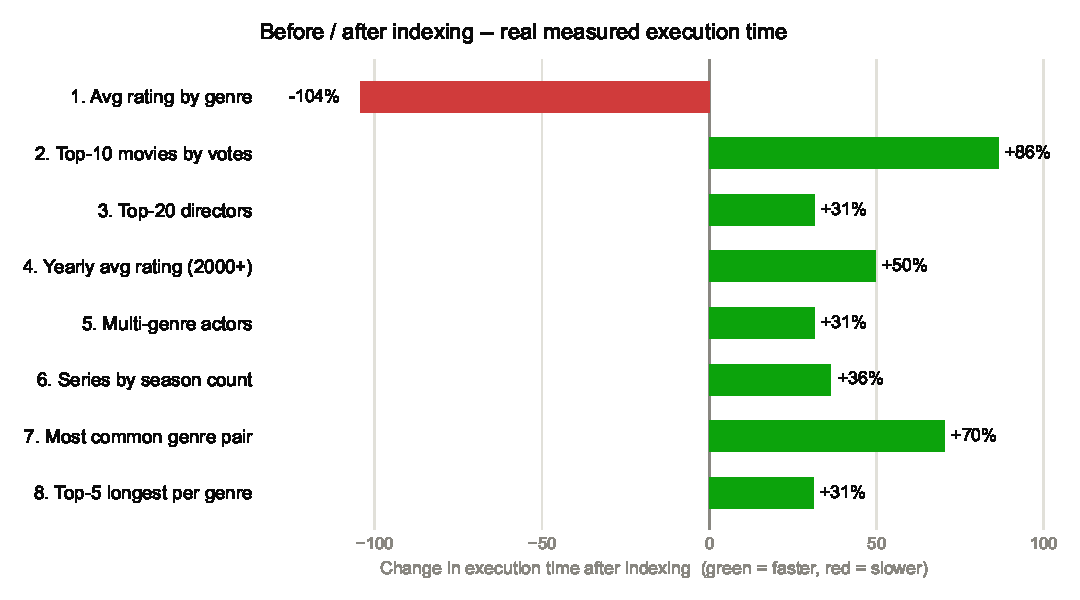
\includegraphics[width=0.85\linewidth]{figures/performance_comparison.pdf}
\caption{همان جدول، به‌صورت نموداری -- درصد تغییر زمان اجرای هر سناریو}
\end{figure}

\paragraph{شش سناریو دقیقاً طبق پیش‌بینی بهتر شدند.} سناریوهای \lr{2}، \lr{4}، \lr{5}، \lr{6}، \lr{7} و \lr{8} همه سریع‌تر شدند. در همه‌ی آن‌ها \lr{Seq Scan} با یک روش ایندکسی (\lr{Index Scan}، \lr{Index Only Scan} یا \lr{Bitmap Heap/Index Scan}) جایگزین شد. بیشترین بهبود مال سناریوی \lr{2} است: از \lr{93} به \lr{12.7} میلی‌ثانیه. ایندکس جزئی \lr{idx\_title\_ratings\_votes\_desc} دقیقاً همان چیزی را می‌دهد که \lr{Top-N} لازم دارد، یعنی مرتب‌سازی کامل حذف می‌شود. نمونه‌ی چشمگیر دیگر سناریوی \lr{8} است: تعداد بلوک خوانده‌شده از دیسک از \lr{115{,}045} به فقط \lr{410} رسید.

\paragraph{سناریوی \lr{3} هنوز کندترین کوئری است -- طبق طراحی.} همان‌طور که در بخش «عمداً بدون ایندکس» گفتیم، هیچ ایندکسی برای ستون \lr{directors} در جدول \lr{title\_crew} نساختیم. این سناریو هم \lr{31\%} سریع‌تر شد، اما این بهبود از خود این تصمیم نیست؛ از تغییری می‌آید که ایندکس‌های \lr{title\_basics} غیرمستقیم روی پیوندهای این کوئری گذاشته‌اند. نکته‌ی جالب این است که این سناریو -- نه سناریوی \lr{5} -- در این اجرا سنگین‌ترین کوئری از آب درآمد. دلیلش همان محدودیت بخش \ref{sec:real-data-scale} است: \lr{title\_crew} و \lr{name\_basics} کامل بارگذاری شدند (\lr{~12.7M} و \lr{~15.5M} سطر)، ولی \lr{title\_principals} فقط \lr{8M} سطر داشت. روی دیتاست کامل \lr{IMDb}، سناریوی \lr{5} احتمالاً دوباره سنگین‌ترین می‌شد، چون از \lr{~90} میلیون سطر \lr{title\_principals} شروع می‌شود.

\paragraph{سناریوی \lr{1} کندتر شد -- و این هم یک نتیجه‌ی واقعی و آموزنده است.} این عدد را مخفی نمی‌کنیم: پلن بعد از ایندکس واقعاً کندتر بود، از \lr{4381} به \lr{8953} میلی‌ثانیه. خود \lr{EXPLAIN} دلیلش را نشان می‌دهد. تعداد بلوک خوانده‌شده از دیسک واقعاً کم شده (از \lr{249{,}303} به \lr{136{,}532})، اما زمان \lr{I/O} واقعی تقریباً دو برابر شده (از حدود \lr{14.9} به \lr{24.9} ثانیه). دلیلش این است که دسترسی از حالت پی‌درپی (در \lr{Parallel Seq Scan}) به دسترسی پراکنده (در \lr{Bitmap Heap Scan}) تغییر کرده.

مشکل اصلی این است که شرط \lr{title\_type = 'movie'} گزینش‌پذیر (\lr{selective}) کافی نیست: نزدیک \lr{30\%} سطرهای \lr{title\_basics} از نوع \lr{movie} هستند. پس \lr{Bitmap Heap Scan} تقریباً به همان تعداد صفحه‌ی دیسک سر می‌زند که یک اسکن کامل می‌زد، ولی با دسترسی پراکنده‌تر و هزینه‌ی اضافه‌ی ساخت بیت‌مپ. درسش ساده است: ایندکس فقط وقتی برنده است که شرط واقعاً گزینشی باشد. روی یک ستون کم‌گزینش مثل \lr{title\_type}، برنامه‌ریز گاهی اشتباه می‌کند؛ برای همین باید همیشه با \lr{EXPLAIN (ANALYZE, BUFFERS)} واقعی تصمیم گرفت، نه فقط با نگاه‌کردن به لیست ایندکس‌ها. (سناریوهای \lr{3}، \lr{5} و \lr{7} هم همین ایندکس \lr{GIN} را برای همین شرط دارند، اما چون شرط دیگری در کوئری‌شان گزینش‌پذیری بیشتری اضافه می‌کند، این اثر منفی آن‌جا دیده نشد.)

\subsection{نمونه‌ی واقعی خروجی \lr{EXPLAIN ANALYZE}}
\label{sec:explain-samples}

خروجی کامل \lr{EXPLAIN (ANALYZE, BUFFERS, SETTINGS)} هر \lr{8} سناریو -- هم قبل و هم بعد از ایندکس‌گذاری، یعنی \lr{16} فایل -- در \Rl{results/explain/} ذخیره شده است. سه نمونه‌ی زیر مستقیماً از همان فایل‌هاست، فقط برای جاشدن در صفحه خلاصه شده‌اند: گره‌های سطح-کارگر و برآورد هزینه‌ی برنامه‌ریز حذف شده‌اند، ولی زمان‌های واقعی و بافرها دست‌نخورده‌اند.

\textbf{سناریوی \lr{1}، قبل و بعد -- همان رگرسیونی که در بالا توضیح داده شد:}

\begin{latin}
\begin{lstlisting}[caption={results/explain/scenario\_01.txt -- BEFORE (excerpt)}]
Sort  (actual time=4347.848..4379.101 rows=27 loops=1)
  Buffers: shared hit=12087 read=249303
  ->  Finalize GroupAggregate  (actual time=4347.418..4378.968 rows=27 loops=1)
        ->  Gather Merge  (Workers Launched: 4)
              ->  Parallel Hash Join  (actual time=2356.150..4191.300 rows=69766 loops=5)
                    ->  Parallel Seq Scan on title_ratings tr
                          (actual time=0.611..1577.639 rows=340413 loops=5)
                    ->  Parallel Seq Scan on title_basics tb
                          Filter: (title_type = 'movie'::text)
                          Rows Removed by Filter: 2387111
                          (actual time=0.596..2089.660 rows=150775 loops=5)
Planning Time: 8.385 ms
Execution Time: 4381.153 ms
\end{lstlisting}
\begin{lstlisting}[caption={results/explain/scenario\_01.after.txt -- AFTER (excerpt)}]
Sort  (actual time=8907.907..8948.027 rows=27 loops=1)
  Buffers: shared hit=69029 read=136532 written=3892
  I/O Timings: shared read=24943.451 write=416.247
  ->  Finalize GroupAggregate  (actual time=8907.699..8947.988 rows=27 loops=1)
        ->  Gather Merge  (Workers Launched: 4)
              ->  Parallel Hash Join  (actual time=6890.573..8659.886 rows=69766 loops=5)
                    ->  Parallel Seq Scan on title_ratings tr
                          (actual time=0.224..1494.175 rows=340413 loops=5)
                    ->  Parallel Bitmap Heap Scan on title_basics tb
                          Recheck Cond: (title_type = 'movie'::text)
                          Heap Blocks: exact=34108
                          (actual time=659.714..6046.800 rows=150775 loops=5)
                          ->  Bitmap Index Scan on idx_title_basics_type_genres_gin
                                (actual time=588.927..588.927 rows=753874 loops=1)
Planning Time: 23.851 ms
Execution Time: 8953.258 ms
\end{lstlisting}
\end{latin}

\textbf{سناریوی \lr{2}، بعد از ایندکس -- بزرگ‌ترین بهبود (از \lr{93} به \lr{12.7} میلی‌ثانیه):}

\begin{latin}
\begin{lstlisting}[caption={results/explain/scenario\_02.after.txt (excerpt)}]
Limit  (actual time=2.379..12.610 rows=10 loops=1)
  Buffers: shared hit=43 read=31
  ->  Nested Loop  (actual time=2.377..12.596 rows=10 loops=1)
        ->  Index Scan using idx_title_ratings_votes_desc on title_ratings tr
              (actual time=1.171..1.235 rows=12 loops=1)
        ->  Index Scan using title_basics_pkey on title_basics tb
              Filter: (title_type = 'movie'::text)
              (actual time=0.939..0.939 rows=1 loops=12)
Planning Time: 7.632 ms
Execution Time: 12.683 ms
\end{lstlisting}
\end{latin}

\textbf{سناریوی \lr{8}، قبل و بعد -- افت بافر خوانده‌شده از \lr{115{,}045} به \lr{410}:}

\begin{latin}
\begin{lstlisting}[caption={results/explain/scenario\_08.txt -- BEFORE, main node only (excerpt)}]
Parallel Seq Scan on title_basics tb  (actual time=2.135..687.571 rows=95056 loops=5)
  Filter: ((runtime_minutes IS NOT NULL) AND (title_type = 'movie'::text))
  Rows Removed by Filter: 2442830
  Buffers: shared hit=115350 read=115044
-- (full plan: Nested Loop -> Sort -> Gather Merge -> WindowAgg above this node)
Execution Time: 2803.599 ms
\end{lstlisting}
\begin{lstlisting}[caption={results/explain/scenario\_08.after.txt (excerpt)}]
Subquery Scan on ranked  (actual time=1079.154..1927.038 rows=135 loops=1)
  Buffers: shared hit=142987 read=410
  ->  WindowAgg  (Run Condition: (row_number() OVER (?) <= 5))
        ->  Nested Loop  (actual time=146.206..477.905 rows=148312 loops=5)
              ->  Parallel Bitmap Heap Scan on title_basics tb
                    Recheck Cond: ((title_type = 'movie'::text) AND
                                    (runtime_minutes IS NOT NULL))
                    (actual time=146.106..382.596 rows=95056 loops=5)
                    ->  Bitmap Index Scan on idx_title_basics_movie_runtime
                          (actual time=91.626..91.626 rows=475280 loops=1)
Planning Time: 5.891 ms
Execution Time: 1930.801 ms
\end{lstlisting}
\end{latin}

\section{مباحث نظری}
\label{sec:theory}

\subsection{پارامترهای تنظیم \lr{PostgreSQL}}

در کنار مستندات رسمی، دو منبع دیگر هم برای تحقیق درباره‌ی این پارامترها مفیدند: \lr{postgresqlco.nf} \cite{pgconfig} که توضیح و مقدار پیش‌فرض هر پارامتر را کنار هم نشان می‌دهد، و \lr{PgTune} \cite{pgtune} که با گرفتن مشخصات سخت‌افزار و نوع بار کاری، یک نقطه‌ی شروع برای این مقادیر پیشنهاد می‌دهد.

\paragraph{\lr{shared\_buffers}.} این پارامتر اندازه‌ی کش مشترک پیج‌های پایگاه‌داده را در حافظه‌ی خود \lr{PostgreSQL} تعیین می‌کند \cite{pgresource}. بزرگ‌کردن زیاد آن همیشه بهتر نیست: چون سیستم‌عامل هم پیج‌ها را در کش خودش نگه می‌دارد، عددی بین \lr{25\%} تا \lr{40\%} حافظه‌ی کل معمولاً خوب است. بیشتر از این، همان داده دوبار (یک‌بار در کش \lr{PostgreSQL}، یک‌بار در کش سیستم‌عامل) نگه داشته می‌شود بدون فایده‌ی اضافه.

\paragraph{\lr{work\_mem}.} برخلاف \lr{shared\_buffers}، این مقدار برای هر عملیات \lr{Sort} یا \lr{Hash} در هر کوئری جداگانه است، نه یک‌بار برای کل سیستم. یک کوئری پیچیده با چند \lr{Sort}/\lr{Hash} می‌تواند چند برابر این مقدار حافظه مصرف کند. پس مقداری که برای یک اتصال خوب است، ممکن است برای صدها اتصال هم‌زمان کل حافظه‌ی سرور را تمام کند. در این پروژه، مقدار سراسری پایین نگه داشته شده و فقط در سطح نشست برای کوئری‌های سنگین بالا می‌رود.

\paragraph{\lr{effective\_cache\_size}.} این پارامتر هیچ حافظه‌ای تخصیص نمی‌دهد؛ فقط یک تخمین به برنامه‌ریز می‌دهد از این‌که چقدر داده احتمالاً در کش جا می‌شود. عدد بزرگ‌تر باعث می‌شود برنامه‌ریز هزینه‌ی \lr{I/O} تصادفی را کمتر تخمین بزند و بیشتر به سمت ایندکس‌ها برود.

\paragraph{\lr{wal\_compression} و \lr{default\_toast\_compression}.} هر دو یک مبادله بین \lr{CPU} و \lr{I/O} دیسک هستند. \lr{lz4} سریع‌تر از الگوریتم پیش‌فرض \lr{pglz} است و روی حجم کاری بارگذاری انبوه این پروژه، هزینه‌ی \lr{CPU} اضافی آن خیلی کمتر از فایده‌ی کاهش نوشتار دیسک است.

\paragraph{\lr{autovacuum}.} \lr{PostgreSQL} از کنترل هم‌روندی چندنسخه‌ای (\lr{MVCC}) استفاده می‌کند: هر \lr{UPDATE}/\lr{DELETE} نسخه‌ی قدیمی سطر را پاک نمی‌کند، فقط آن را «مرده» علامت می‌زند تا تراکنش‌های دیگر که هنوز به آن نیاز دارند خراب نشوند. \lr{autovacuum} این سطرهای مرده را پاک می‌کند. آستانه‌ی پیش‌فرض آن (درصدی از اندازه‌ی جدول) برای یک صف کار که خیلی سریع‌تر از رشد جدول، سطر مرده تولید می‌کند مناسب نیست؛ به همین دلیل جدول \lr{message\_queue} با آستانه‌ی مطلق (تعداد ثابت سطر) تنظیم شده، نه آستانه‌ی نسبی.

\paragraph{\lr{maintenance\_work\_mem}.} این پارامتر هم مثل \lr{work\_mem} یک محدودیت حافظه است، ولی نه برای کوئری‌های معمولی؛ برای عملیات‌های نگه‌داری مثل \lr{CREATE INDEX}، \lr{VACUUM} و \lr{ALTER TABLE} استفاده می‌شود. چون این عملیات‌ها معمولاً یکی‌یکی و کم‌تعداد اجرا می‌شوند، نه هم‌زمان برای صدها اتصال مثل \lr{work\_mem}، می‌شود مقدار آن را خیلی بزرگ‌تر گذاشت بدون نگرانی از تمام‌شدن حافظه‌ی سرور. مقدار پیش‌فرض \lr{PostgreSQL} فقط \lr{64MB} است؛ برای پروژه‌ای که باید ایندکس یک جدول \lr{90} میلیون سطری بسازد، این عدد کم است -- عدد بزرگ‌تر یعنی مرتب‌سازی ساخت ایندکس در حافظه انجام شود، نه با چند پاس روی دیسک. به همین دلیل در این پروژه \lr{768MB} گذاشته شده.

\paragraph{\lr{wal\_buffers}.} قبل از این‌که رکوردهای \lr{WAL} (لاگ پیش‌نوشت، برای بازیابی بعد از کرش) واقعاً روی دیسک نوشته شوند، اول در یک بافر مشترک در حافظه جمع می‌شوند؛ این پارامتر اندازه‌ی همان بافر است. مقدار پیش‌فرض آن \lr{-1} است، یعنی خودکار تنظیم شود (معمولاً حدود \lr{1/32} از \lr{shared\_buffers}). بزرگ‌ترکردن آن به تراکنش‌های هم‌زمان زیاد کمک می‌کند، چون رکوردهای بیشتری قبل از یک نوشتار واقعی جمع می‌شوند؛ ولی بعد از یک حد مشخص (اندازه‌ی چیزی که بین دو چک‌پوینت واقعاً نوشته می‌شود) بزرگ‌ترکردن بیشتر فایده‌ای ندارد. در این پروژه روی \lr{16MB} تنظیم شده.

\paragraph{\lr{min\_wal\_size} و \lr{max\_wal\_size}.} این دو، فضایی که \lr{PostgreSQL} برای فایل‌های \lr{WAL} نگه می‌دارد را کنترل می‌کنند و مستقیماً روی زمان‌بندی چک‌پوینت اثر می‌گذارند. رسیدن حجم \lr{WAL} به \lr{max\_wal\_size} باعث می‌شود یک چک‌پوینت زودتر از موعد اجرا شود. \lr{max\_wal\_size} کوچک یعنی چک‌پوینت‌های مکرر -- هزینه‌ی \lr{I/O} بیشتر ولی بازیابی سریع‌تر بعد از کرش؛ \lr{max\_wal\_size} بزرگ یعنی چک‌پوینت‌های کم‌تر -- برای بارگذاری انبوه بهتر است، ولی بازیابی بعد از کرش کندتر می‌شود. مقدار پیش‌فرض \lr{PostgreSQL 16} برای این دو به‌ترتیب \lr{80MB} و \lr{1GB} است. در این پروژه، عمداً یک \lr{max\_wal\_size} نسبتاً کوچک (\lr{4GB}) انتخاب شده تا خط پایه رفتار واقعی یک بارگذاری \lr{I/O}-محدود را نشان دهد.

\paragraph{\lr{seq\_page\_cost} و \lr{random\_page\_cost}.} این دو، واحد هزینه‌ای هستند که برنامه‌ریز کوئری برای مقایسه‌ی پلن‌های مختلف استفاده می‌کند: \lr{seq\_page\_cost} هزینه‌ی خواندن یک صفحه به‌صورت پی‌درپی است (پیش‌فرض \lr{1.0})، و \lr{random\_page\_cost} هزینه‌ی خواندن یک صفحه به‌صورت تصادفی (پیش‌فرض \lr{4.0}). این نسبت \lr{4} به \lr{1} از دنیای دیسک‌های مکانیکی می‌آید، جایی که یک جهش تصادفی سر دیسک واقعاً چند برابر کندتر از خواندن پی‌درپی بود. روی \lr{SSD}/\lr{NVMe} این تفاوت خیلی کمتر است، پس نگه‌داشتن \lr{random\_page\_cost} روی \lr{4} باعث می‌شود برنامه‌ریز به‌اشتباه فکر کند ایندکس همیشه گران‌تر از اسکن کامل است. در این پروژه \lr{random\_page\_cost} روی \lr{1.1} تنظیم شده تا با واقعیت سخت‌افزار سازگار باشد.

\paragraph{\lr{enable\_seqscan}، \lr{enable\_indexscan} و \lr{enable\_bitmapscan}.} این سه، کلید قطع‌ووصل سطح-نشست هستند؛ خاموش‌کردن هرکدام آن روش دسترسی را کاملاً ممنوع نمی‌کند، فقط هزینه‌ی آن را مصنوعی خیلی بالا می‌برد تا برنامه‌ریز تقریباً همیشه از آن فرار کند. کاربرد اصلی‌شان تست و مقایسه است، نه تنظیم دائمی در \lr{postgresql.conf}: مثلاً می‌شود موقتاً \lr{enable\_bitmapscan} را خاموش کرد تا ببینیم اگر ایندکس در دسترس نبود پلن چه شکلی می‌شد، بدون این‌که واقعاً ایندکس را حذف کنیم.

ما همین کار را واقعاً برای سناریوی \lr{1} (بخش \ref{sec:indexing}) انجام دادیم: با \lr{enable\_bitmapscan = off} و \lr{enable\_indexscan = off}، برنامه‌ریز مجبور شد به‌جای \lr{Bitmap Heap Scan} (که خودش انتخاب کرده بود، در \lr{8953.3} میلی‌ثانیه) به \lr{Parallel Seq Scan} برگردد -- این‌بار در \lr{14522.6} میلی‌ثانیه، یعنی حتی کندتر. نکته‌ی مهم: این عدد را نباید مستقیم با عدد اصلی «قبل از ایندکس» (\lr{4381.2} میلی‌ثانیه) مقایسه کرد، چون آن اندازه‌گیری ساعت‌ها زودتر و با کش تازه‌تری از دیسک انجام شده بود؛ اما مقایسه‌ی این دو عدد در همین نشست (هردو با وضعیت کش یکسان) نشان می‌دهد که برنامه‌ریز، با توجه به کش فعلی، واقعاً بهترین گزینه‌ی موجود را انتخاب کرده بود -- فقط آن گزینه از عدد خط پایه‌ی اصلی بدتر بود.

\subsection{مقایسه‌ی انواع ایندکس}

\begin{itemize}
\item \textbf{\lr{B-Tree}} (پیش‌فرض \lr{PostgreSQL}): یک ساختار درختی که کلیدها را مرتب نگه می‌دارد. برای تساوی، بازه (\lr{<}, \lr{>}, \lr{BETWEEN}) و مرتب‌سازی خوب است. فقط ستون‌های اول یک ایندکس چندستونی قابل‌استفاده‌اند.
\item \textbf{\lr{Hash}}: فقط برای تساوی (\lr{=}) خوب است؛ نه بازه و نه مرتب‌سازی را پشتیبانی نمی‌کند. از \lr{PostgreSQL 10} به بعد بعضی وقت‌ها کوچک‌تر و سریع‌تر از \lr{B-Tree} است، اما این مزیت به‌ندرت به‌اندازه‌ای است که ارزش از دست‌دادن بازه/مرتب‌سازی را داشته باشد -- به همین دلیل در این پروژه استفاده نشده.
\item \textbf{\lr{GiST}} (\lr{Generalized Search Tree}): برخلاف بقیه که برای یک نوع داده‌ی خاص طراحی شده‌اند، \lr{GiST} یک چارچوب عمومی است. با نوشتن چندتابع خاص (تشخیص هم‌پوشانی، فشرده‌سازی، ادغام)، می‌شود آن را برای داده‌های خیلی متفاوت به‌کار برد: داده‌ی هندسی/جغرافیایی (مثلاً در \lr{PostGIS})، بازه‌ها (\lr{range types})، جست‌وجوی نزدیک‌ترین همسایه (\lr{KNN}، با عملگر \lr{<->})، و حتی جست‌وجوی متن به‌عنوان جایگزین \lr{GIN}. ساخت و به‌روزرسانی آن معمولاً سریع‌تر از \lr{GIN} است، ولی چون بعضی از پیاده‌سازی‌هایش \lr{lossy} هستند (ممکن است نتیجه‌ی اضافی هم برگردد که باید دوباره چک شود)، جست‌وجو در آن کمی کندتر و اندازه‌اش بزرگ‌تر از یک \lr{GIN} هم‌ارز است.
\item \textbf{\lr{GIN}} (\lr{Generalized Inverted Index}): برای مقادیری که هر سطر چندتا از آن‌ها دارد -- آرایه، \lr{JSONB}، جست‌وجوی متن. برای هر مقدار داخلی، یک لیست از سطرهایی که آن مقدار را دارند نگه می‌دارد. برای «آیا این مقدار توی این ستون هست؟» (\lr{@>}, \lr{\&\&}) خیلی سریع است، اما مفهوم ترتیب ندارد و فقط با \lr{Bitmap Index Scan} در دسترس است، نه \lr{Index Scan} ساده. با پسوند \lr{btree\_gin}، یک \lr{GIN} می‌تواند چند ستون از نوع‌های مختلف را با هم ترکیب کند و -- برخلاف \lr{B-Tree} -- با فیلتر روی هرکدام از این ستون‌ها به‌تنهایی هم کار کند.
\item \textbf{\lr{BRIN}} (\lr{Block Range Index}): برای ستون‌هایی که ترتیب فیزیکی‌شان روی دیسک با ترتیب مقدارشان همخوانی دارد (مثلاً یک ستون زمانی که به‌ترتیب درج شده) خیلی کوچک و کم‌هزینه است، چون فقط بازه‌ی مقدار هر بلوک دیسک را نگه می‌دارد، نه هر سطر را. در این پروژه استفاده نشده چون داده‌ی \lr{IMDb} بعد از عبور از صف پیام، دیگر لزوماً با همان ترتیبی که \lr{BRIN} لازم دارد درج نمی‌شود.
\end{itemize}

\paragraph{کدام ایندکس برای \lr{JSONB} مناسب است؟} از این چهار نوع، \lr{GIN} انتخاب استاندارد \lr{PostgreSQL} برای \lr{JSONB} است -- همان‌طور که بالا گفته شد، دقیقاً برای سؤال «آیا این کلید/مقدار توی این \lr{JSONB} هست؟» (\lr{@>}, \lr{?}) طراحی شده. \lr{GiST} هم روی \lr{JSONB} قابل‌استفاده است ولی رایج نیست و معمولاً کندتر از \lr{GIN} عمل می‌کند. \lr{B-Tree} و \lr{Hash} اصلاً مناسب این کار نیستند، چون فقط تساوی/ترتیب کل مقدار \lr{JSONB} را می‌فهمند، نه محتوای داخلش را.

\subsection{\lr{JSONB} و مکانیزم \lr{TOAST}}

\paragraph{تفاوت \lr{JSON} و \lr{JSONB}.} نوع \lr{JSON} متن خام ورودی را دقیقاً همان‌طور که نوشته شده نگه می‌دارد -- با همان فاصله‌ها، همان ترتیب کلیدها، و حتی کلیدهای تکراری. هر بار که این مقدار خوانده یا پرس‌وجو شود، \lr{PostgreSQL} باید کل متن را از نو تجزیه (\lr{parse}) کند. \lr{JSONB} برعکس این است: در زمان نوشتن یک‌بار تجزیه و به یک قالب باینری آماده تبدیل می‌شود. نتیجه یک مبادله‌ی ساده است: درج \lr{JSONB} کمی کندتر است (چون باید ساخته شود)، ولی خواندن و جست‌وجو خیلی سریع‌تر است (چون تجزیه‌ی دوباره لازم نیست) -- برای همین تقریباً همیشه \lr{JSONB} به \lr{JSON} ترجیح داده می‌شود.

\paragraph{\lr{JSONB} چگونه در داخل \lr{PostgreSQL} ذخیره می‌شود؟} مقدار \lr{JSONB} به‌صورت یک قالب باینریِ از قبل تجزیه‌شده و «تجزیه‌شده» (\lr{decomposed binary format}) ذخیره می‌شود، نه به‌صورت متن. این قالب یک هدر به همراه آرایه‌ای از افست‌ها/طول‌ها دارد که مستقیماً به محل هر کلید و مقدار در همان مقدار باینری اشاره می‌کند. کلیدهای هر شیء بر اساس طول و سپس ترتیب بایتی مرتب نگه داشته می‌شوند، پس پیداکردن یک کلید مشخص با جست‌وجوی دودویی (\lr{binary search}) روی همین آرایه ممکن است -- بدون این‌که کل مقدار از اول خوانده شود. سه چیز در این فرایند تبدیل از بین می‌رود: فاصله‌های خالی متن اصلی، ترتیب اصلی کلیدها (چون بر اساس طول/بایت دوباره مرتب می‌شوند)، و کلیدهای تکراری (اگر یک کلید دوبار در ورودی بیاید، فقط آخرین مقدارش نگه داشته می‌شود). اعداد هم به‌جای متن، در یک نوع عددی داخلی ذخیره می‌شوند. همین ساختار باینریِ با افستِ مستقیم است که هم جست‌وجوی سریع را ممکن می‌کند و هم پایه‌ی ساخت ایندکس \lr{GIN} روی \lr{JSONB} است.

\paragraph{عملگرها و توابع مهم \lr{JSONB}.} چندتای پرکاربردش: \lr{->} یک فیلد/عضو را به‌صورت \lr{jsonb} برمی‌گرداند؛ \lr{->>} همان را به‌صورت متن برمی‌گرداند؛ \lr{@>} می‌پرسد «آیا سمت چپ شامل سمت راست است؟» -- همان عملگر \lr{containment} که ایندکس \lr{GIN} برایش ساخته می‌شود؛ \lr{?} می‌پرسد «آیا این کلید در سطح بالای \lr{JSONB} وجود دارد؟». از توابع هم \lr{jsonb\_set()} (تغییر یک مقدار داخلی بدون خواندن-تغییر-نوشتن کل شیء در کد برنامه)، \lr{jsonb\_agg()} (جمع‌کردن چند سطر در یک آرایه‌ی \lr{JSONB}) و \lr{jsonb\_each()} (باز کردن یک \lr{JSONB} به سطرهای کلید-مقدار) پرکاربردند. در این پروژه، ستون \lr{title\_ratings.metadata} دقیقاً با عملگر \lr{@>} قابل‌پرس‌وجوست -- مثلاً \lr{metadata @> '\{"popular": true\}'} که روی داده‌ی واقعی این پروژه \lr{17{,}906} سطر برمی‌گرداند.

\lr{TOAST} (\lr{The Oversized-Attribute Storage Technique}) \cite{pgtoast} مکانیزمی است که به \lr{PostgreSQL} اجازه می‌دهد مقادیر متغیرطول بزرگ (مثل \lr{JSONB}، متن یا آرایه) را بیرون از سطر اصلی، در یک جدول کمکی نگه دارد. چهار روش ذخیره برای هر ستون وجود دارد: \lr{PLAIN} (بدون فشرده‌سازی یا انتقال؛ برای انواع با اندازه‌ی ثابت)، \lr{MAIN} (فشرده‌سازی درون‌خطی، انتقال به بیرون فقط اگر واقعاً لازم باشد)، \lr{EXTENDED} (پیش‌فرض \lr{JSONB}؛ هم فشرده‌سازی هم انتقال به بیرون مجاز است) و \lr{EXTERNAL} (بدون فشرده‌سازی ولی انتقال به بیرون مجاز -- برای وقتی که دسترسی تصادفی به بخشی از مقدار مهم‌تر از فضاست). فعال‌شدن این مکانیزم -- همان‌طور که در بخش \ref{sec:queue} گفتیم -- بر اساس کل سطر است، نه هر ستون؛ همین نکته پایه‌ی طراحی بسته‌بندی دسته‌ای این پروژه است.

\paragraph{ساخت ایندکس \lr{GIN} روی \lr{JSONB}.} دستور ساده است: \lr{CREATE INDEX ... ON table USING GIN (jsonb\_column)}. حالت پیش‌فرض (\lr{jsonb\_ops}) هم کلیدها هم مقدارها را ایندکس می‌کند و از \lr{@>}, \lr{?}, \lr{?|}, \lr{?\&} پشتیبانی می‌کند. یک گزینه‌ی دیگر، \lr{jsonb\_path\_ops}، فقط از \lr{@>} پشتیبانی می‌کند ولی ایندکس کوچک‌تر و سریع‌تری می‌سازد -- برای ستونی مثل \lr{metadata} در این پروژه که (اگر روزی لازم شود) فقط قرار است با \lr{containment} پرس‌وجو شود، \lr{jsonb\_path\_ops} انتخاب بهتری از پیش‌فرض بود.

\paragraph{\lr{JSONB} یا جدول نرمال‌شده؟} قاعده‌ی ساده: اگر قرار است روی یک فیلد داخلی زیاد فیلتر/پیوند/گروه‌بندی کنید، بهتر است آن فیلد یک ستون واقعی با ایندکس \lr{B-Tree} باشد -- برنامه‌ریز آمار بهتری از یک ستون واقعی دارد تا از داخل یک \lr{JSONB}. اما اگر ساختار داده متغیر است (هر سطر ممکن است کلیدهای متفاوتی داشته باشد)، یا قرار است کل شیء با هم خوانده/نوشته شود، \lr{JSONB} بهتر است چون از ساختن چندین جدول کمکی با ستون‌های اغلب \lr{NULL} جلوگیری می‌کند. ستون \lr{metadata} در این پروژه دقیقاً نمونه‌ی دوم است: داده‌ی مشتق‌شده‌ای که هیچ‌کدام از هشت سناریو روی آن فیلتر نمی‌کند، پس نیازی به نرمال‌سازی ندارد.

\subsection{نظریه‌ی صف پیام}

\paragraph{الگوی \lr{Competing Consumers}.} در این الگو، چند مصرف‌کننده‌ی مستقل از یک صف مشترک کار برمی‌دارند تا پردازش سریع‌تر شود. مشکل اصلی این است که یک کار نباید توسط بیش از یک مصرف‌کننده برداشته شود، بدون این‌که مصرف‌کننده‌ها مجبور شوند پشت سر هم صف بکشند.

\paragraph{مکانیزم \lr{LISTEN}/\lr{NOTIFY}.} این دو دستور، مکانیزم داخلی \lr{PostgreSQL} برای اطلاع‌رسانی بین نشست‌ها هستند. یک نشست با \lr{LISTEN channel\_name} روی یک کانال ثبت‌نام می‌کند؛ هر نشست دیگری با \lr{NOTIFY channel\_name, 'payload'} (یا تابع \lr{pg\_notify}) یک پیام کوتاه متنی به همه‌ی نشست‌های ثبت‌نام‌شده روی آن کانال می‌فرستد -- این پیام معمولاً بعد از \lr{commit} همان تراکنش، به‌صورت غیرهم‌زمان به گیرنده‌ها می‌رسد.

\paragraph{چرا \lr{LISTEN}/\lr{NOTIFY} به‌تنهایی برای صف کافی نیست.} مشکل اصلی این است که \lr{NOTIFY} هیچ حافظه‌ای ندارد: اگر لحظه‌ی ارسال هیچ نشستی روی آن کانال گوش نمی‌داد، آن پیام برای همیشه گم می‌شود -- نه صف‌بندی، نه امکان بازپخش. همچنین \lr{NOTIFY} به‌صورت پخش (\lr{broadcast}) به همه‌ی گوش‌دهنده‌ها می‌رسد، نه فقط یکی؛ یعنی خودش هیچ تضمینی نمی‌دهد که یک پیام دقیقاً یک‌بار توسط یکی از مصرف‌کننده‌ها برداشته شود -- دقیقاً همان مشکلی که \lr{Competing Consumers} باید حلش کند. به همین دلیل این پروژه، حالت واقعی صف (وضعیت، مهلت، شمارنده‌ی تلاش) را در جدول \lr{message\_queue} نگه می‌دارد، نه در \lr{NOTIFY}. اگر لازم شود، می‌شود \lr{LISTEN}/\lr{NOTIFY} را فقط به‌عنوان یک زنگ‌خطر سبک اضافه کرد -- مصرف‌کننده به‌جای \lr{polling} دوره‌ای منتظر \lr{NOTIFY} بماند -- ولی وضعیت واقعی هر پیام همچنان باید در جدول بماند.

\paragraph{\lr{SKIP LOCKED} در برابر قفل معمولی.} یک \lr{SELECT ... FOR UPDATE} معمولی، اگر سطرهایش قبلاً قفل شده باشند، منتظر می‌ماند تا آزاد شوند -- یعنی مصرف‌کننده‌ها پشت سر هم صف می‌کشند. اضافه‌کردن \lr{SKIP LOCKED} \cite{pglocking} این رفتار را عوض می‌کند: هر سطر قفل‌شده از نتیجه حذف می‌شود و تراکنش می‌رود سراغ سطر آزاد بعدی. نتیجه این است که \lr{N} مصرف‌کننده‌ی هم‌زمان، \lr{N} دسته‌ی کاملاً جدا از صف برمی‌دارند، بدون این‌که منتظر هم بمانند -- دقیقاً همان چیزی که \lr{Competing Consumers} نیاز دارد.

\paragraph{تضمین‌های تحویل.} سه سطح رایج وجود دارد: \lr{at-most-once} (پیام ممکن است هیچ‌وقت پردازش نشود، ولی هیچ‌وقت هم دوبار پردازش نمی‌شود)، \lr{at-least-once} (پیام حتماً حداقل یک‌بار پردازش می‌شود، ولی ممکن است در بعضی حالت‌ها -- مثلاً خرابی مصرف‌کننده قبل از تأیید -- بیش از یک‌بار هم پردازش شود)، و \lr{exactly-once} (که در سیستم‌های توزیع‌شده‌ی واقعی، بدون یک لایه‌ی هماهنگ‌کننده‌ی اضافه، تقریباً غیرممکن یا خیلی گران است). صف این پروژه تضمین \lr{at-least-once} می‌دهد: مکانیزم مهلت با \lr{locked\_until} تضمین می‌کند اگر مصرف‌کننده‌ای قبل از \lr{ack} از کار بیفتد، پیام (بعد از تمام‌شدن مهلت و اجرای \lr{reap\_expired}) دوباره به صف برمی‌گردد -- ولی این یعنی ممکن است همان پیام دوبار پردازش شود.

\paragraph{بی‌اثری (\lr{Idempotency}).} چون تضمین \lr{at-least-once} اجازه می‌دهد پردازش تکراری اتفاق بیفتد، مصرف‌کننده باید طوری طراحی شود که پردازش دوباره‌ی یک پیام، نتیجه‌ی نهایی را عوض نکند. در این پروژه، این کار با \lr{ON CONFLICT DO NOTHING} روی کلید اصلی هر جدول انجام شده: اگر یک دسته دوبار درج شود (مثلاً به‌خاطر برگشتن به صف)، تلاش دوم سطرهای تکراری را نادیده می‌گیرد، بدون خطا و بدون تغییر داده.

\paragraph{جدول-به‌عنوان-صف در برابر راه‌حل تخصصی.} همان‌طور که پروژه‌ی \lr{Postgres For Everything} \cite{pgeverything} هم نشان می‌دهد، \lr{PostgreSQL} می‌تواند نقش خیلی از ابزارهای تخصصی -- از جمله صف پیام -- را بازی کند. استفاده از یک جدول ساده به‌جای یک \lr{message broker} تخصصی (مثل \lr{RabbitMQ} یا \lr{Kafka}) چند مزیت دارد: هیچ زیرساخت جدیدی لازم نیست، و از همه مهم‌تر، می‌شود \lr{enqueue} کردن یک پیام و تغییر بقیه‌ی داده‌ها را در یک تراکنش واحد انجام داد -- یک \lr{broker} جدا این هماهنگی رایگان را نمی‌دهد. عیبش این است که زیر بار خیلی سنگین (هزاران تولیدکننده/مصرف‌کننده هم‌زمان) به‌اندازه‌ی یک \lr{broker} تخصصی مقیاس‌پذیر نیست، و هر بار \lr{poll} یک کوئری واقعی روی همان پایگاه‌داده‌ای است که به کارهای دیگر هم سرویس می‌دهد؛ ویژگی‌های پیشرفته‌تر (مسیریابی پیچیده، بازپخش از یک نقطه‌ی مشخص، داشبورد نظارتی) هم باید از صفر ساخته شوند. برای حجم کار این پروژه -- یک بارگذاری انبوه، نه پیام‌رسانی بین چند سرویس مستقل -- سادگی جدول-به‌عنوان-صف کاملاً کافی و حتی ترجیح داده می‌شود.

\section{نتیجه‌گیری}
\label{sec:conclusion}

این پروژه یک معماری کامل برای بارگذاری و کوئری‌گرفتن از مجموعه‌داده‌ی \lr{IMDb} روی \lr{PostgreSQL 16} ساخت: یک صف پیام با \lr{SELECT ... FOR UPDATE SKIP LOCKED} برای بارگذاری هم‌زمان و بدون رقابت، بسته‌بندی دسته‌ای برای رد کردن آستانه‌ی فشرده‌سازی \lr{TOAST}، هشت سناریوی کوئری طبق سند پروژه، و شش ایندکس که هرکدام به یک شرط مشخص در این سناریوها وصل است.

هر بخش از این پروژه -- اسکیمای پایگاه‌داده، توابع صف، تولیدکننده و مصرف‌کننده، کوئری‌ها، و طراحی ایندکس -- حداقل یک‌بار با یک بازبینی چندعاملی بررسی شده و باگ‌های واقعی پیداشده در آن اصلاح شده‌اند. برای بخش‌هایی که نیازی به اجرای واقعی نداشتند (نحو \lr{SQL}، منطق \lr{Python}، تست‌های خودکار)، درستی با ابزارهایی مثل \lr{py\_compile} و آزمون دستی چک شده است.

\subsection{محدودیت این نگارش}

همه‌ی عددهای بخش \ref{sec:indexing} از یک اجرای واقعی \lr{PostgreSQL 16} داخل \lr{Docker} به دست آمده‌اند، نه از پیش‌بینی. تنها محدودیت واقعی این اجرا فضای دیسک بود: لپ‌تاپی که این پروژه رویش اجرا شد فقط حدود \lr{30} گیگابایت فضای خالی داشت، و بیشتر از این هم نمی‌شد جا باز کرد. دیتاست کامل \lr{IMDb} -- مخصوصاً جدول \lr{title\_principals} با نزدیک \lr{90} میلیون سطر -- توی این فضا جا نمی‌شد. برای همین فقط همین یک جدول با فلگ \lr{--limit-rows} به \lr{8} میلیون سطر (حدود \lr{9\%}) محدود شد؛ شش جدول دیگر کامل بارگذاری شدند (جزئیات در بخش \ref{sec:real-data-scale}). نتیجه‌ی عملی این محدودیت این است که سناریوی \lr{5} -- تنها سناریویی که از \lr{title\_principals} می‌خواند -- روی حجمی کوچک‌تر از واقعیت سنجیده شده؛ بهبود واقعی آن روی دیتاست کامل احتمالاً بیشتر از عدد گزارش‌شده است.

یک نتیجه‌ی دیگر هم ارزش گفتن دارد: ایندکس \lr{GIN} ترکیبی، سناریوی \lr{1} را کندتر کرد نه سریع‌تر. این عدد را حذف یا نرم نکردیم، چون خودش یک درس واقعی از این پروژه است. ایندکس‌گذاری فقط با نگاه‌کردن به لیست شرط‌های کوئری کافی نیست. باید با \lr{EXPLAIN (ANALYZE, BUFFERS)} واقعی سنجید، چون گزینش‌پذیری کم یک شرط -- مثل \lr{title\_type = 'movie'} -- می‌تواند نتیجه‌ی برعکس بدهد.

\subsection{کارهای آینده}

اگر بخواهیم این پروژه را گسترش دهیم، سه مسیر طبیعی برای ادامه وجود دارد: افراز کردن (\lr{partitioning}) جدول \lr{title\_principals} بر اساس \lr{category} برای کم‌کردن بیشتر حجم اسکن‌شده در سناریوی \lr{5}؛ استفاده از دیدهای مادی‌شده (\lr{materialized views}) برای سناریوهایی که به‌طور دوره‌ای اجرا می‌شوند نه بلادرنگ؛ و پایش مستمر عملکرد با \lr{pg\_stat\_statements} برای پیدا کردن خودکار کوئری‌هایی که با تغییر داده در طول زمان، به ایندکس یا تنظیم جدیدی نیاز پیدا می‌کنند.


\begin{thebibliography}{9}

\bibitem{pgdocs}
\lr{PostgreSQL Global Development Group}, «\lr{PostgreSQL 16 Documentation}»,
\lr{\url{https://www.postgresql.org/docs/16/index.html}}

\bibitem{pgtoast}
\lr{PostgreSQL Global Development Group}, «\lr{TOAST (The Oversized-Attribute Storage Technique)}»,
\lr{\url{https://www.postgresql.org/docs/16/storage-toast.html}}

\bibitem{pggin}
\lr{PostgreSQL Global Development Group}, «\lr{GIN Indexes}»,
\lr{\url{https://www.postgresql.org/docs/16/gin.html}}

\bibitem{pglocking}
\lr{PostgreSQL Global Development Group}, «\lr{SELECT ... FOR UPDATE SKIP LOCKED}»,
\lr{\url{https://www.postgresql.org/docs/16/sql-select.html\#SQL-FOR-UPDATE-SKIP-LOCKED}}

\bibitem{pgresource}
\lr{PostgreSQL Global Development Group}, «\lr{Resource Consumption (\lr{shared\_buffers}, \lr{work\_mem}, ...)}»,
\lr{\url{https://www.postgresql.org/docs/16/runtime-config-resource.html}}

\bibitem{pgconfig}
\lr{postgresqlco.nf}, «\lr{PostgreSQL Configuration Documentation}»,
\lr{\url{https://postgresqlco.nf/}}

\bibitem{pgtune}
\lr{PgTune}, «\lr{PostgreSQL Configuration Calculator}»,
\lr{\url{https://pgtune.leopard.in.ua/}}

\bibitem{pgeverything}
\lr{Daniel Olshansky}, «\lr{Postgres For Everything}»,
\lr{\url{https://github.com/olshansk/postgres_for_everything}}

\bibitem{imdb}
\lr{IMDb}, «\lr{IMDb Non-Commercial Datasets}»,
\lr{\url{https://datasets.imdbws.com/}}

\bibitem{imdbdocs}
\lr{IMDb}, «\lr{Non-Commercial Datasets -- Documentation}»,
\lr{\url{https://developer.imdb.com/non-commercial-datasets/}}

\end{thebibliography}

\end{document}
